% ****** Start of file apssamp.tex ******
%
%   This file is part of the APS files in the REVTeX 4.2 distribution.
%   Version 4.2a of REVTeX, December 2014
%
%   Copyright (c) 2014 The American Physical Society.
%
%   See the REVTeX 4 README file for restrictions and more information.
%
% TeX'ing this file requires that you have AMS-LaTeX 2.0 installed
% as well as the rest of the prerequisites for REVTeX 4.2
%
% See the REVTeX 4 README file
% It also requires running BibTeX. The commands are as follows:
%
%  1)  latex apssamp.tex
%  2)  bibtex apssamp
%  3)  latex apssamp.tex
%  4)  latex apssamp.tex
%
\documentclass[%
 % reprint,
10pt,
superscriptaddress,
twocolumn,
%groupedaddress,
%unsortedaddress,
%runinaddress,
%frontmatterverbose,
%preprint,
%preprintnumbers,
%nofootinbib,
%nobibnotes,
%bibnotes,
 amsmath,amssymb,
 aps,prx,
%pra,
%prb,
%rmp,
%prstab,
%prstper,
%floatfix,
]{revtex4-2}

\usepackage{graphicx}% Include figure files
\usepackage{dcolumn}% Align table columns on decimal point
\usepackage{bm}% bold math
\usepackage{xcolor}
\usepackage{hyperref}% add hypertext capabilities
\usepackage{siunitx}% SI units
\usepackage{physics}
\usepackage[utf8]{inputenc}
\usepackage[T1]{fontenc}
\usepackage{lmodern}
\usepackage{amsmath,amsfonts,amssymb}


\AtBeginDocument{\renewcommand*{\d}{\mathop{\kern0pt\mathrm{d}}\!{}}}
\graphicspath{{Figures/}} % set default figure path to figures/, if we store figure files in figures/, we only need to put file name in \includegraphics{filename.pdf}. For supported formats, e.g. pdf and jpg, we can omit the extensions. This enhances the readability of the source.

% Some formatting guidelines
% 1. Start a new line (\n) for each sentence. This is good for synctex (click pdf and find the line in tex), and also good for Git when comparing versions.
% 2. Communicate thoughts in comments. For example, if you think a figure of something is needed but missing some where, put a comment and describe the needs.
% 3. Colored text: I use red text to emphasize that the claim is not fully backed by our results. The wording may be modified in the future.
% 4. Figure crossref: at the beginning of a sentence, use "Figure~\ref{}". Otherwise, use "Fig.~\ref{}". Note that the "~" is to prevent line breaking in the middle of the crossref.

% Some content problems that need to be fixed
% 1. Same quantities are referred to in different notations, e.g. \tau^* and \tilde{\tau}, x and y, \tilde{D} and D_A



\begin{document}

\preprint{APS/123-QED}

\title{Active Nematics at Bifurcations}% Force line breaks with \\



\author{Zhengyang Liu}
\author{Claire Doré}
\affiliation{Laboratoire Gulliver, UMR 7083 CNRS, ESPCI Paris, PSL Research University, 75005 Paris, France.}

\author{Antonio Tavera-Vazquez}
\affiliation{Laboratoire Gulliver, UMR 7083 CNRS, ESPCI Paris, PSL Research University, 75005 Paris, France.}
\affiliation{Pritzker School of Molecular Engineering, University of Chicago, Chicago, IL 60637, USA.}

\author{Teresa Lopez-Leon}
\affiliation{Laboratoire Gulliver, UMR 7083 CNRS, ESPCI Paris, PSL Research University, 75005 Paris, France.}
\date{\today}
% It is always \today, today,
%  but any date may be explicitly specified




\begin{abstract}

Under lateral confinement, active matter self-organize into coherent flows. 
Such behavior implies the possibility of achieving logical operations in properly designed channel networks. 
Bifurcations are a key ingredient in channel networks.
Understanding active matter behavior at bifurcations is therefore an important step towards a proper channel network design.
In this paper, we experimentally explore active matter behavior at bifurcations using the microtubule-kinesin model system. 
Specifically, we compare the effects of channel length, ratchets and turning angles. 
Our results suggest that ratchets and turning angles help establish unambiguous polarized flow states.
In contrast, channel length is a less relevant factor, which results in more frequently changing flow states.
Our experiment is the first step to study active matter behavior in complex channel networks in the simplest form.
The resutls lay the foundation for realizing networks that can achieve active matter logic and computation.

\end{abstract}

%\keywords{Suggested keywords}%Use showkeys class option if keyword
                              %display desired
\maketitle

\section{Introduction}

Active fluids flow spontaneously under channel confinement, a phenomenon observed in various active matter systems \cite{Lushi2014,Wioland2016,Wu2017,Duclos2017,Morin2018,Hardouin2020} followed by a theoretical prediction \cite{Voituriez2005}.
Without addressing the detailed mechanisms that govern the magnitude of the spontaneous flow, \citet{Woodhouse2017} proposed to use a Landau-type bistable potential to model the phenomenon. Combining some other ingredients, such as incompressibility and diode channel, they derived rich and interesting behaviors of active flow networks (AFN), including active matter logic \cite{Woodhouse2016,Woodhouse2017}.

Networks are topologically more complex than channels. 
The most notable feature is nodes connecting more than two channels, in particular odd number of channels. 
According to the model by \citet{Woodhouse2017} and the experiment by \citet{Morin2018}, all channels have a preferred flow rate $\phi_0$, given the same channel width and activity.
However, when three channels are connected to one node, imcompressibility frustrates the flow state where flow rates in all the channels are $\phi_0$.
In such a frustrated state, the model by \citet{Woodhouse2017} predicts that the most favorable flow state is that the flow enters the node at flow rate $\phi_0$ from one channel and exits at the same flow rate $\phi_0$ through another channel, leaving the flow rate in the third channel $0$.
Furthermore, if the two outlet channels are of different lengths, the exit flow follows the longer path.  
This behavior is the fundation to achieve logical operation with active matter confined in channel networks. 

We find it interesting to realize active flow networks in experiment. 
First, this realization provides a playground to test and improve existing theories, and thus deepen our understanding of active matter behavior in complex environment. 
Second, this realization lays the foundation for potential applications of active flow networks in mass transport and flow computation. 
However, experimental realization of AFN is very rare due to the technical challenges in fabricating and properly applying the confinement structure to active matter.
\textcolor{red}{In particular, the networks are open in 2D, which requires 3D confinement structure, making traditional photolithography technique challenging.}

In this work, we take advantage of a two-photon polymerization based high-precision 3D printing to fabricate open network structures (see Fig.~\ref{fig:bifurcation-experiment}b). 
We use microtubule-kinesin system as the model active matter to experimentally test all the ingredients in the theory of AFN, namely bistable potential, incompressibility and diode channel. 
Then, we use these ingredients to predict and understand more complicated bifurcation experiments.
Our results suggest that ratchets and turning angles help establish unambiguous polarized flow states.
In contrast, channel length is a less relevant factor, which results in more frequently changing flow states.
Our experiment is the first step to study active matter behavior in complex channel networks in the simplest form.
The resutls lay the foundation for realizing networks that can achieve active matter logic and computation.

  
\begin{figure}[!h]
    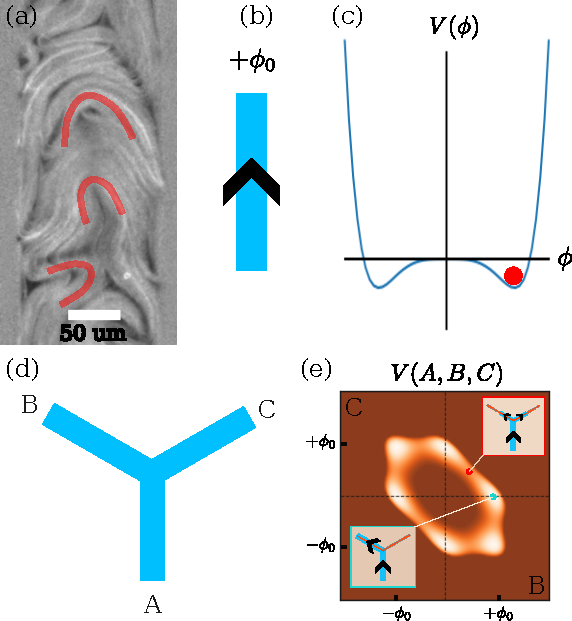
\includegraphics[width=0.45\textwidth]{1-bifurcation-question}
    \caption{
    \textbf{What do active nematics do in straight channels and bifurcations?}
    (a) Spontaneous directed flow in a straight channel.
    (b) A schematic diagram of the directed flow in a straight channel.
    (c) Energy landscape of flow rate in a straight channel predicted by a Landau-type phenomenological model, relating flow potential $V(\phi)$ and flow rate $\phi$ of active flows. 
    The red disk represents the most probable flow in the positive direction, corresponding to the scenario in a and b.
    (d) A schematic diagram of three interconnected straight channels, the so called ``bifurcation''.
    (e) Energy landscape of the flow rate configurations in the bifurcation. 
    The blue dot and the lower left inset illustrate a typical ``polarized'' flow state, where the in-coming flow from one channel completely goes into one of the two outlet channels without splitting. 
    The red dot and the upper right inset illustrate a typical ``non-polarized'' flow state, where the in-coming flow from one channel equally splits the two outlet channels. 
    }
    \label{fig:bifurcation-question}
\end{figure}

\section{Experiment}

\begin{figure}[!h]
    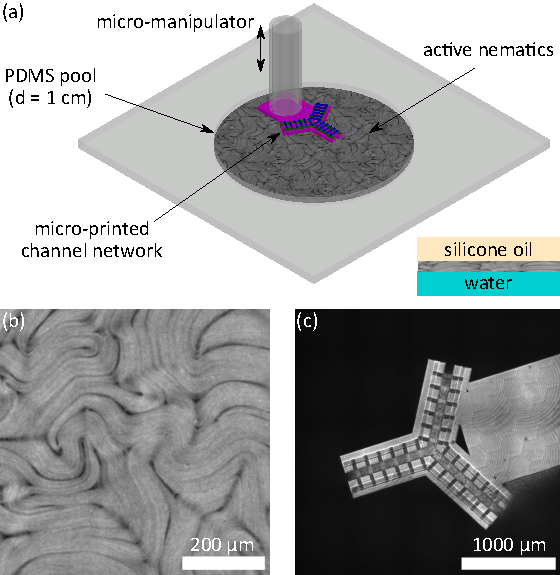
\includegraphics[width=0.45\textwidth]{2-bifurcation-experiment}
    \caption{
    \textbf{Confining microtubule-kinesin system at water-oil inerface -- the experimental setup.}
    (a) A schematic diagram of the experimental setup. 
    The microtubule-kinesin active nematic system is condensed at the water-oil interface, and is subject to lateral confinement by nano-printed channels. 
    (b) A schematic diagram of the bifurcation channels. 
    The Y-shape channel pattern is printed at the bottom.
    The ``bridges'' on the top are designed to hold the structure together. 
    (c) Top view of the bifurcation channels. 
    The relevant dimensions channel length $l=1000$ $\mu$m and channel width $w=100$ $\mu$m are labeled in place. 
    (d) A confocal image of a mature interfacial microtubule-kinesin system. 
    (e) A confocal image of the bifurcation channels set on the interfacial microtubule-kinesin system. 
    }
    \label{fig:bifurcation-experiment}
\end{figure}


\begin{figure*}[!h]
    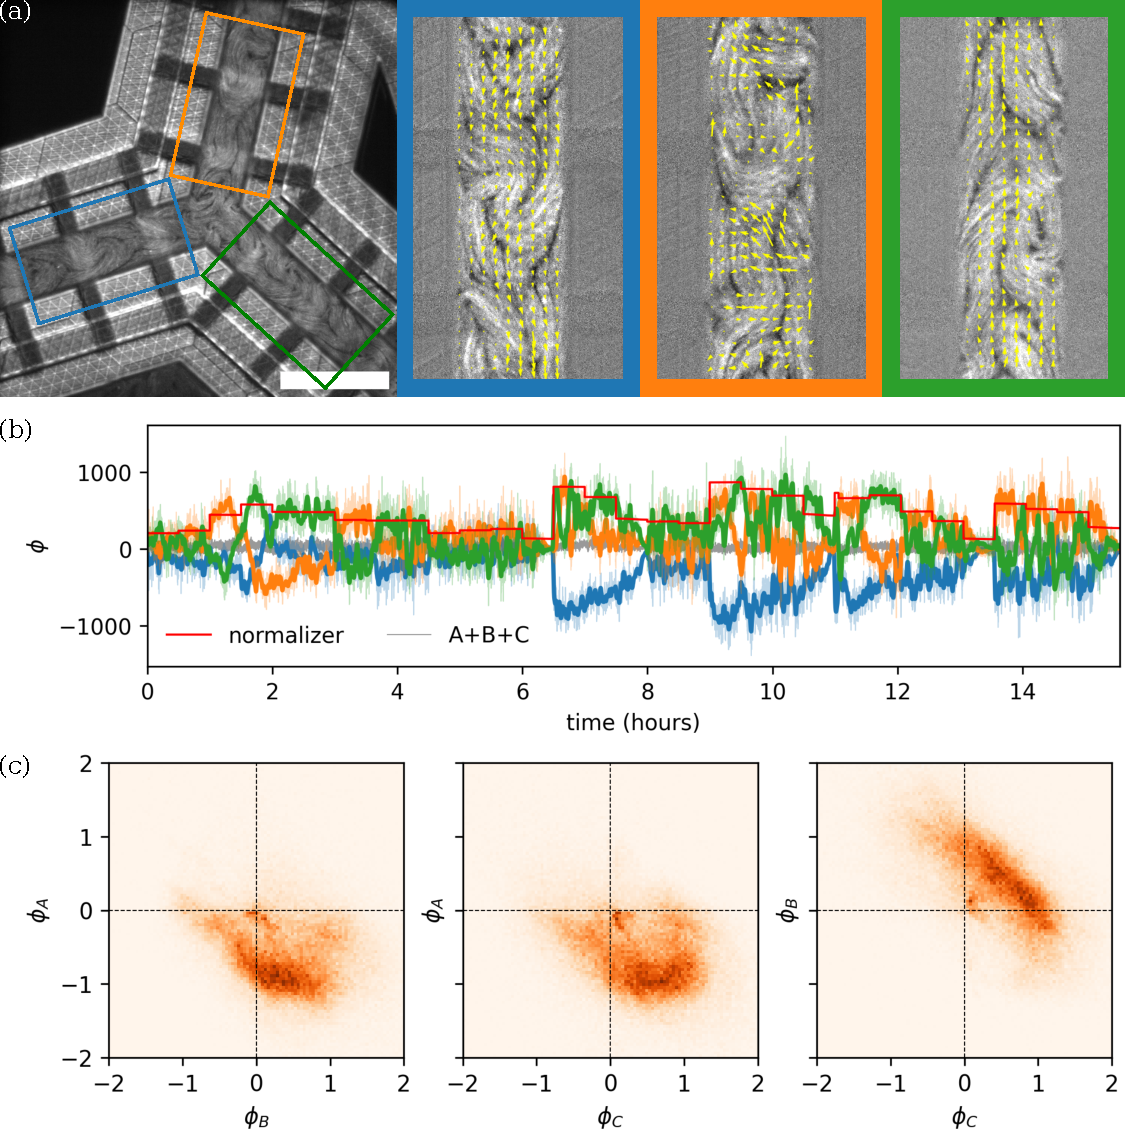
\includegraphics[width=\textwidth]{3-bifurcation-symmetric}
    \caption{
    \textbf{Flow rate measurements and flow rate histogram.}
    (a) A snapshot of microtubule-kinesin system at a bifurcation.
    The 3 panels on the right are crops of each channel with corresponding border colors. 
    The yellow arrows are the results from PIV analysis. 
    (b) Flow rate time series in the 3 channels A (blue), B (orange) and C (green). 
    The light and thin curves in the back are the real flow rates, while the strong and thick curves in the front are Gaussian-smoothed flow rates with $\sigma=25$ s. 
    The red curve is the ``normalizer'', defined as the maximum of the   smoothed absoluted flow rates in A, B and C. 
    The gray curve is the sum of the flow rates in the 3 channels, which is used to verify the continuity at the junction.
    The unit of flow rate is $\mu$m$^2$/s.
    Note that the direction away from the junction is defined as the positive direction. 
    (c) The histogram of normalized flow rates. From left to right $\phi_A$-$\phi_B$, $\phi_A$-$\phi_C$ and $\phi_B$-$\phi_C$. Note that these histograms are not independent since the 3 flow rates satisfy $\phi_A+\phi_B+\phi_C = 0$. Therefore, in the following, we only show $\phi_B$-$\phi_C$ histogram.
    }
    \label{fig:bifurcation-symmetric}
\end{figure*}

\section{Results}

\begin{figure*}[!h]
    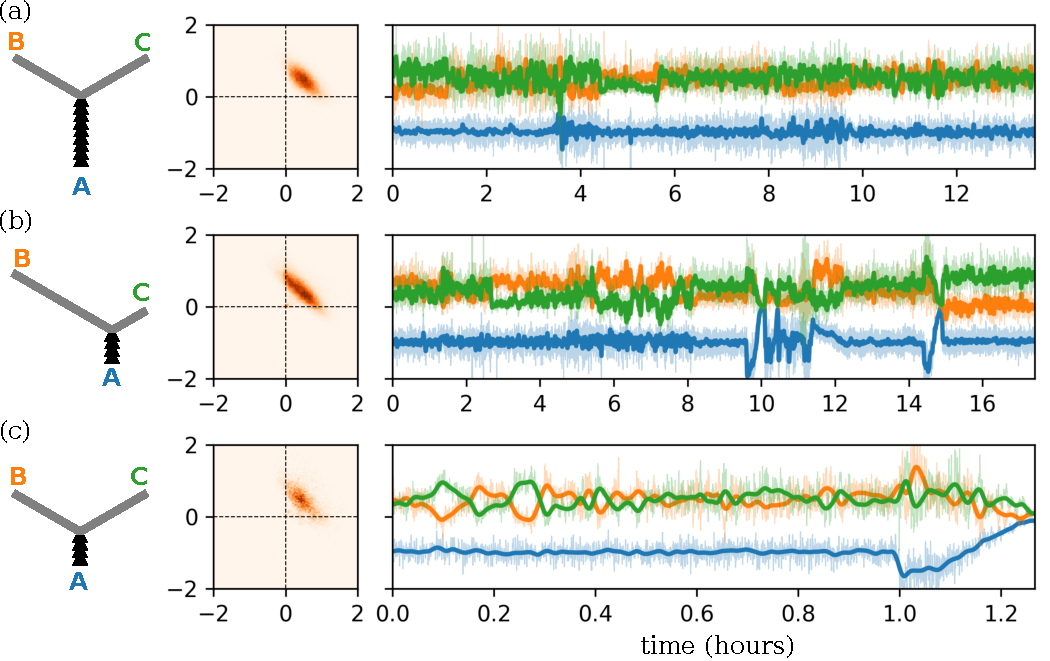
\includegraphics[width=\textwidth]{4-straight-channel-length}
    \caption{
    \textbf{Ratchet inlet and straight outlets: histogram and time series.}
    (a) 9-teeth ratchet inlet with 2 equal length outlets. 
    The flow fluctuates between polarized and non-polarized states, exploring all the possible configurations.
    The equal splitting state is the most probable configuration.
    (b) 4-teeth ratchet inlet with long and short outlets.
    The flow also explores all the possible configurations, but shows no preferred splitting ratio.
    (c) 4-teeth ratchet inlet with 2 equal length outlets.
    The flow fluctuates between polarized and non-polarized states, exploring all the possible configurations.
    The equal splitting state is the most probable configuration.
    }
    \label{fig:straight-channel-length}
\end{figure*}

\begin{figure*}[!h]
    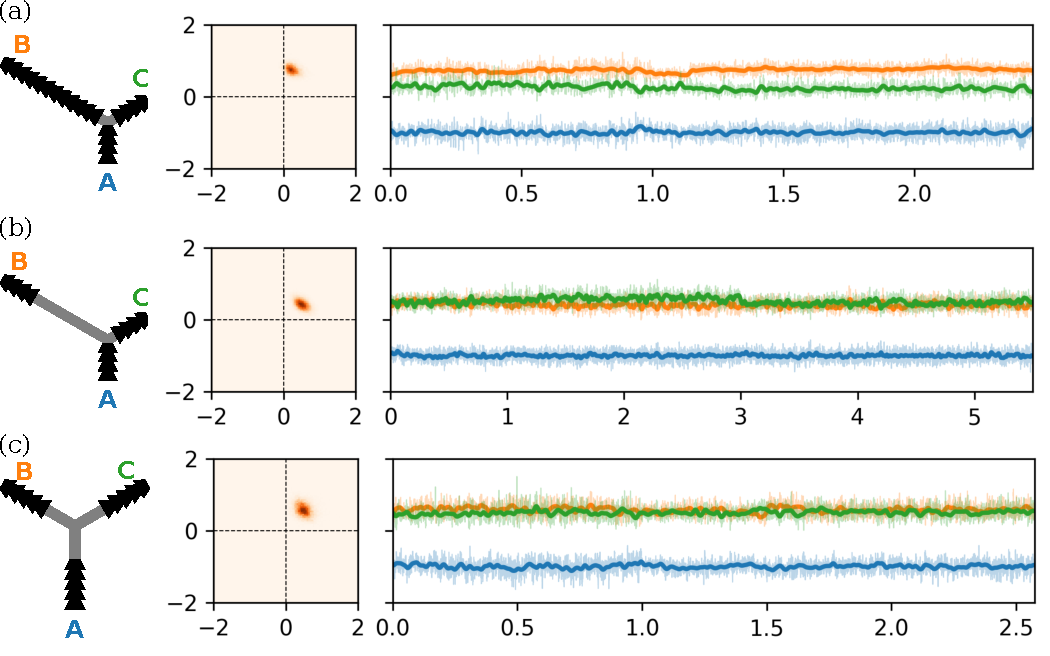
\includegraphics[width=\textwidth]{5-ratchet-dominance}
    \caption{
    \textbf{Ratchet inlet and outlets: histogram and time series.}
    (a) The numbers of ratchet teeth in channels A, B and C are 4, 13 and 4, respectively. 
    Let's refer to this bifurcation channel network 4-13-4 bifurcation. 
    In contrast to straight channels, the flows exhibit a sharp peak in the histogram, while other splitting ratios remain rarely explored. 
    The splitting ratio is around 3:1.
    (b) 4-4-4 bifurcation, where channel B has an extended straight portion. 
    The flows again exhibit a sharp peak in the histogram at a splitting ratio around 1:1.
    (c) 5-5-5 bifurcation, where all the channels are of the same length. 
    The flows again exhibit a sharp peak in the histogram at a splitting ratio around 1:1.
    }
    \label{fig:ratchet-dominance}
\end{figure*}

\begin{figure*}[!h]
    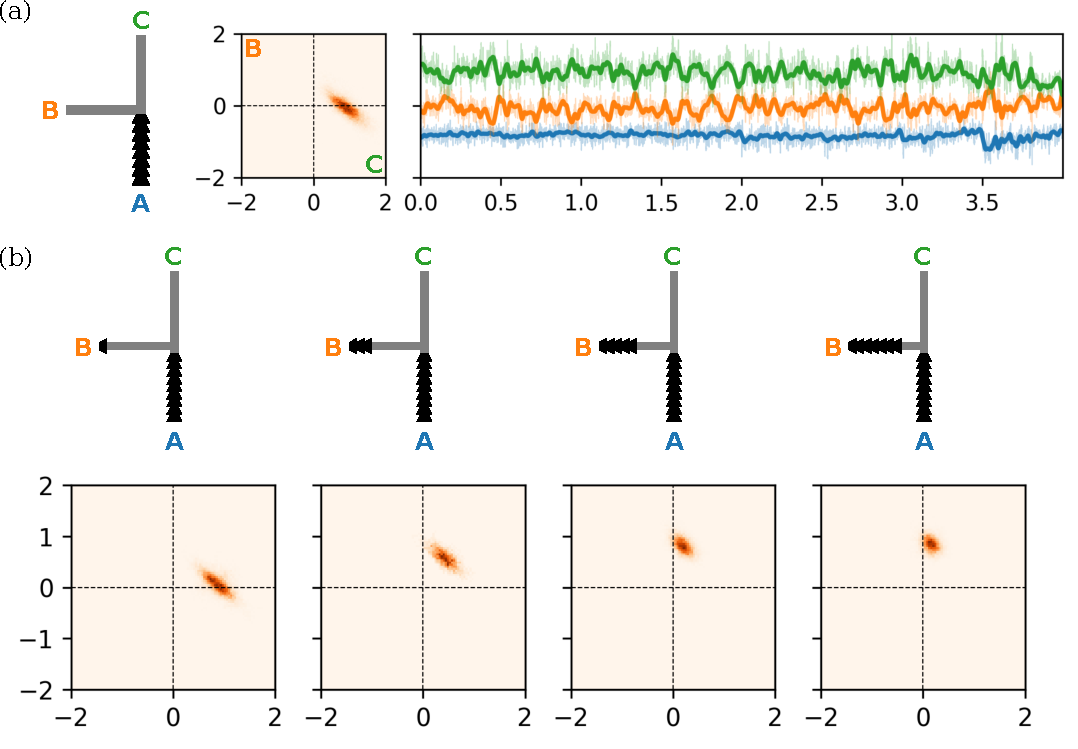
\includegraphics[width=\textwidth]{6-angle-ratchet-competition}
    \caption{
    \textbf{The role of turning angles.}
    (a) A bifurcation with a 9-teeth ratchet inlet and 2 straight outlets of the same length. 
    The outlets have different turning angles with respect to the inlet channel A: $\angle AOB=90^\circ$ and $\angle AOC=180^\circ$.
    The flow rate histogram and time series suggest that the flow prefers the $180^\circ$ channel C, i.e. the channel parallel to the inlet channel A, rather than channel B which requires a $90^\circ$ turn. 
    (b) Adding various numbers of ratchets to channel B to compete with the $90^\circ$ turning angle. 
    From left to right, 1, 3, 5, 7 ratchet teeth are added to the end of channel B. 
    Below the schematics of bifurcation channels are the $\phi_B$-$\phi_C$ flow rate histograms corresponding to the design above. 
    As the number of ratchet teeth in channel B is increased, the splitting ratio between B and C is increase from 0 to $\infty$.
    }
    \label{fig:angle-ratchet-competition}
\end{figure*}

\bibliography{ref}



\end{document}
%
% ****** End of file apssamp.tex ******